
\definecolor{white}{RGB}{255,255,255}
\definecolor{cffda00}{RGB}{255,218,0}
\definecolor{cb26b00}{RGB}{178,107,0}
\definecolor{cff9900}{RGB}{255,153,0}
\definecolor{yellow}{RGB}{255,255,0}
\definecolor{cb28e00}{RGB}{178,142,0}
\definecolor{cffcc00}{RGB}{255,204,0}


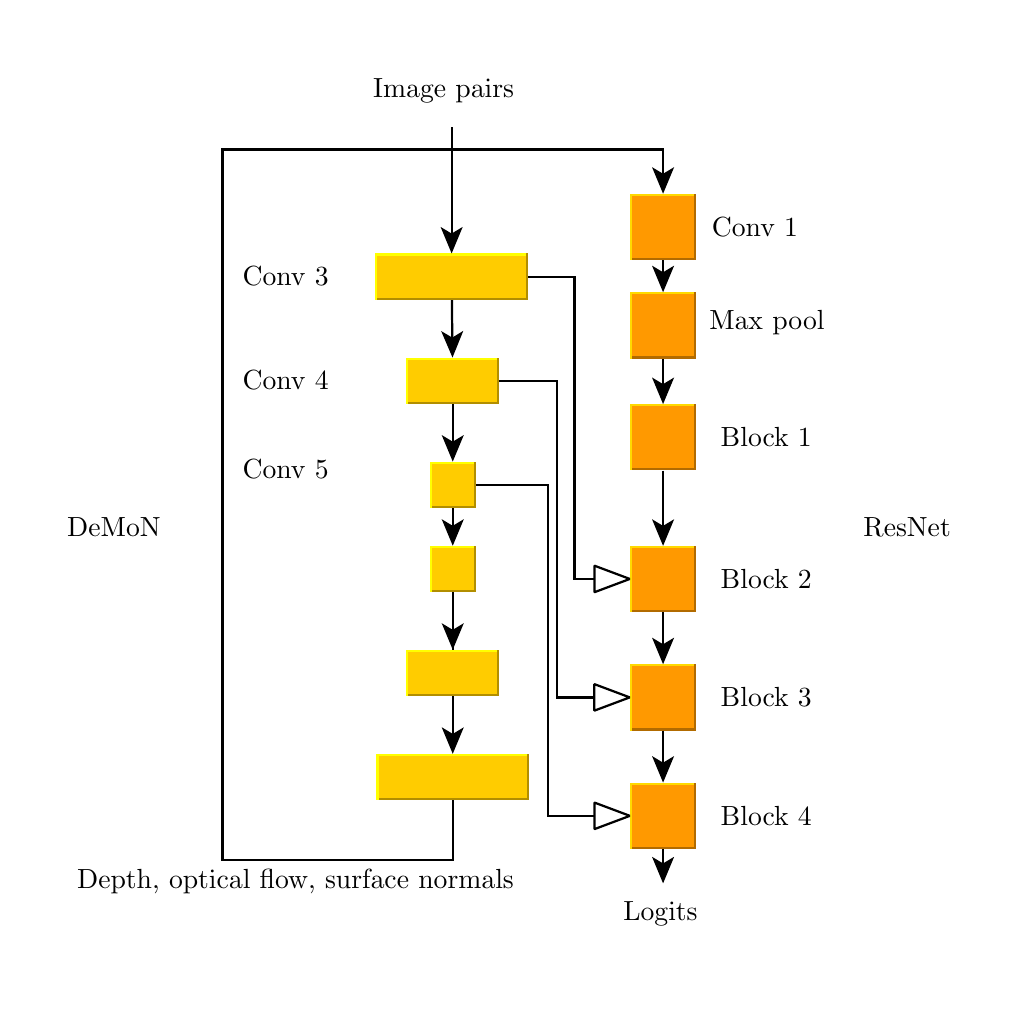
\begin{tikzpicture}[y=0.80pt, x=0.80pt, yscale=-1.000000, xscale=1.000000, inner sep=0pt, outer sep=0pt,
draw=black,fill=black,line join=miter,line cap=rect,miter limit=10.00,line width=0.800pt]
  \begin{scope}[shift={(-474.0,27.0)},draw=white,fill=white]
    \path[fill,rounded corners=0.0000cm] (474.0000,-27.0000) rectangle
      (912.0000,405.0000);
  \end{scope}
  \begin{scope}[cm={{1.0,0.0,0.0,1.0,(-474.0,27.0)}},draw=cff9900,fill=cff9900]
    \path[fill,rounded corners=0.0000cm] (746.0000,48.0000) rectangle
      (776.0000,78.0000);
    \path[fill=cffda00,rounded corners=0.0000cm] (746.0000,48.0000) rectangle
      (747.0000,78.0000);
    \path[fill=cffda00,rounded corners=0.0000cm] (747.0000,48.0000) rectangle
      (775.0000,49.0000);
    \path[fill=cb26b00,rounded corners=0.0000cm] (747.0000,77.0000) rectangle
      (776.0000,78.0000);
    \path[fill=cb26b00,rounded corners=0.0000cm] (775.0000,48.0000) rectangle
      (776.0000,77.0000);
  \end{scope}
  \begin{scope}[cm={{1.0,0.0,0.0,1.0,(-474.0,27.0)}},line cap=butt,miter limit=1.45]
    \path[fill] (783.0615,67.1543) node[above right] (text4014) {Conv 1};
  \end{scope}
  \begin{scope}[cm={{1.0,0.0,0.0,1.0,(-474.0,27.0)}},draw=cff9900,fill=cff9900]
    \path[fill,rounded corners=0.0000cm] (746.0000,92.5000) rectangle
      (776.0000,122.5000);
    \path[fill=cffda00,rounded corners=0.0000cm] (746.0000,92.5000) rectangle
      (747.0000,122.5000);
    \path[fill=cffda00,rounded corners=0.0000cm] (747.0000,92.5000) rectangle
      (775.0000,93.5000);
    \path[fill=cb26b00,rounded corners=0.0000cm] (747.0000,121.5000) rectangle
      (776.0000,122.5000);
    \path[fill=cb26b00,rounded corners=0.0000cm] (775.0000,92.5000) rectangle
      (776.0000,121.5000);
  \end{scope}
  \begin{scope}[cm={{1.0,0.0,0.0,1.0,(-474.0,27.0)}},line cap=butt,miter limit=1.45]
    \path[fill] (781.8711,111.6543) node[above right] (text4030) {Max pool};
  \end{scope}
  \begin{scope}[cm={{1.0,0.0,0.0,1.0,(-474.0,27.0)}},draw=cff9900,fill=cff9900]
    \path[fill,rounded corners=0.0000cm] (746.0000,143.0000) rectangle
      (776.0000,173.0000);
    \path[fill=cffda00,rounded corners=0.0000cm] (746.0000,143.0000) rectangle
      (747.0000,173.0000);
    \path[fill=cffda00,rounded corners=0.0000cm] (747.0000,143.0000) rectangle
      (775.0000,144.0000);
    \path[fill=cb26b00,rounded corners=0.0000cm] (747.0000,172.0000) rectangle
      (776.0000,173.0000);
    \path[fill=cb26b00,rounded corners=0.0000cm] (775.0000,143.0000) rectangle
      (776.0000,172.0000);
  \end{scope}
  \begin{scope}[cm={{1.0,0.0,0.0,1.0,(-474.0,27.0)}},line cap=butt,miter limit=1.45]
    \path[fill] (787.0479,162.1543) node[above right] (text4046) {Block 1};
  \end{scope}
  \begin{scope}[cm={{1.0,0.0,0.0,1.0,(-474.0,27.0)}},draw=cff9900,fill=cff9900]
    \path[fill,rounded corners=0.0000cm] (746.0000,207.0000) rectangle
      (776.0000,237.0000);
    \path[fill=cffda00,rounded corners=0.0000cm] (746.0000,207.0000) rectangle
      (747.0000,237.0000);
    \path[fill=cffda00,rounded corners=0.0000cm] (747.0000,207.0000) rectangle
      (775.0000,208.0000);
    \path[fill=cb26b00,rounded corners=0.0000cm] (747.0000,236.0000) rectangle
      (776.0000,237.0000);
    \path[fill=cb26b00,rounded corners=0.0000cm] (775.0000,207.0000) rectangle
      (776.0000,236.0000);
  \end{scope}
  \begin{scope}[cm={{1.0,0.0,0.0,1.0,(-474.0,27.0)}},line cap=butt,miter limit=1.45]
    \path[fill] (787.0479,226.1543) node[above right] (text4062) {Block 2};
  \end{scope}
  \begin{scope}[cm={{1.0,0.0,0.0,1.0,(-474.0,27.0)}},draw=cff9900,fill=cff9900]
    \path[fill,rounded corners=0.0000cm] (746.0000,260.5000) rectangle
      (776.0000,290.5000);
    \path[fill=cffda00,rounded corners=0.0000cm] (746.0000,260.5000) rectangle
      (747.0000,290.5000);
    \path[fill=cffda00,rounded corners=0.0000cm] (747.0000,260.5000) rectangle
      (775.0000,261.5000);
    \path[fill=cb26b00,rounded corners=0.0000cm] (747.0000,289.5000) rectangle
      (776.0000,290.5000);
    \path[fill=cb26b00,rounded corners=0.0000cm] (775.0000,260.5000) rectangle
      (776.0000,289.5000);
  \end{scope}
  \begin{scope}[cm={{1.0,0.0,0.0,1.0,(-474.0,27.0)}},line cap=butt,miter limit=1.45]
    \path[fill] (787.0479,279.6543) node[above right] (text4078) {Block 3};
  \end{scope}
  \begin{scope}[cm={{1.0,0.0,0.0,1.0,(-474.0,27.0)}},draw=cff9900,fill=cff9900]
    \path[fill,rounded corners=0.0000cm] (746.0000,314.0000) rectangle
      (776.0000,344.0000);
    \path[fill=cffda00,rounded corners=0.0000cm] (746.0000,314.0000) rectangle
      (747.0000,344.0000);
    \path[fill=cffda00,rounded corners=0.0000cm] (747.0000,314.0000) rectangle
      (775.0000,315.0000);
    \path[fill=cb26b00,rounded corners=0.0000cm] (747.0000,343.0000) rectangle
      (776.0000,344.0000);
    \path[fill=cb26b00,rounded corners=0.0000cm] (775.0000,314.0000) rectangle
      (776.0000,343.0000);
  \end{scope}
  \begin{scope}[cm={{1.0,0.0,0.0,1.0,(-474.0,27.0)}},line cap=butt,miter limit=1.45]
    \path[fill] (787.0479,333.1543) node[above right] (text4094) {Block 4};
  \end{scope}
  \begin{scope}[cm={{1.0,0.0,0.0,1.0,(-474.0,27.0)}},draw=cffcc00,fill=cffcc00]
    \path[fill,rounded corners=0.0000cm] (631.0000,75.0000) rectangle
      (700.0000,96.0000);
    \path[fill=yellow,rounded corners=0.0000cm] (631.0000,75.0000) rectangle
      (632.0000,96.0000);
    \path[fill=yellow,rounded corners=0.0000cm] (632.0000,75.0000) rectangle
      (699.0000,76.0000);
    \path[fill=cb28e00,rounded corners=0.0000cm] (632.0000,95.0000) rectangle
      (700.0000,96.0000);
    \path[fill=cb28e00,rounded corners=0.0000cm] (699.0000,75.0000) rectangle
      (700.0000,95.0000);
  \end{scope}
  \begin{scope}[cm={{1.0,0.0,0.0,1.0,(-474.0,27.0)}},line cap=butt,miter limit=1.45]
    \path[fill] (851.4814,202.6543) node[above right] (text4110) {ResNet};
  \end{scope}
  \begin{scope}[cm={{1.0,0.0,0.0,1.0,(-474.0,27.0)}},draw=cffcc00,fill=cffcc00]
    \path[fill,rounded corners=0.0000cm] (645.0000,122.0000) rectangle
      (687.0000,143.0000);
    \path[fill=yellow,rounded corners=0.0000cm] (645.0000,122.0000) rectangle
      (646.0000,143.0000);
    \path[fill=yellow,rounded corners=0.0000cm] (646.0000,122.0000) rectangle
      (686.0000,123.0000);
    \path[fill=cb28e00,rounded corners=0.0000cm] (646.0000,142.0000) rectangle
      (687.0000,143.0000);
    \path[fill=cb28e00,rounded corners=0.0000cm] (686.0000,122.0000) rectangle
      (687.0000,142.0000);
    \path[fill,rounded corners=0.0000cm] (655.5000,169.0000) rectangle
      (676.5000,190.0000);
    \path[fill=yellow,rounded corners=0.0000cm] (655.5000,169.0000) rectangle
      (656.5000,190.0000);
    \path[fill=yellow,rounded corners=0.0000cm] (656.5000,169.0000) rectangle
      (675.5000,170.0000);
    \path[fill=cb28e00,rounded corners=0.0000cm] (656.5000,189.0000) rectangle
      (676.5000,190.0000);
    \path[fill=cb28e00,rounded corners=0.0000cm] (675.5000,169.0000) rectangle
      (676.5000,189.0000);
    \path[fill,rounded corners=0.0000cm] (655.5000,207.0000) rectangle
      (676.5000,228.0000);
    \path[fill=yellow,rounded corners=0.0000cm] (655.5000,207.0000) rectangle
      (656.5000,228.0000);
    \path[fill=yellow,rounded corners=0.0000cm] (656.5000,207.0000) rectangle
      (675.5000,208.0000);
    \path[fill=cb28e00,rounded corners=0.0000cm] (656.5000,227.0000) rectangle
      (676.5000,228.0000);
    \path[fill=cb28e00,rounded corners=0.0000cm] (675.5000,207.0000) rectangle
      (676.5000,227.0000);
    \path[fill,rounded corners=0.0000cm] (645.0000,254.0000) rectangle
      (687.0000,275.0000);
    \path[fill=yellow,rounded corners=0.0000cm] (645.0000,254.0000) rectangle
      (646.0000,275.0000);
    \path[fill=yellow,rounded corners=0.0000cm] (646.0000,254.0000) rectangle
      (686.0000,255.0000);
    \path[fill=cb28e00,rounded corners=0.0000cm] (646.0000,274.0000) rectangle
      (687.0000,275.0000);
    \path[fill=cb28e00,rounded corners=0.0000cm] (686.0000,254.0000) rectangle
      (687.0000,274.0000);
    \path[fill,rounded corners=0.0000cm] (631.5000,301.0000) rectangle
      (700.5000,322.0000);
    \path[fill=yellow,rounded corners=0.0000cm] (631.5000,301.0000) rectangle
      (632.5000,322.0000);
    \path[fill=yellow,rounded corners=0.0000cm] (632.5000,301.0000) rectangle
      (699.5000,302.0000);
    \path[fill=cb28e00,rounded corners=0.0000cm] (632.5000,321.0000) rectangle
      (700.5000,322.0000);
    \path[fill=cb28e00,rounded corners=0.0000cm] (699.5000,301.0000) rectangle
      (700.5000,321.0000);
  \end{scope}
  \begin{scope}[cm={{1.0,0.0,0.0,1.0,(-474.0,27.0)}},line cap=butt,miter limit=1.45]
    \path[fill] (571.0615,89.6543) node[above right] (text4166) {Conv 3};
    \path[fill] (571.0615,136.6543) node[above right] (text4168) {Conv 4};
    \path[fill] (571.0615,176.6699) node[above right] (text4170) {Conv 5};
    \path[fill] (491.8525,202.6543) node[above right] (text4172) {DeMoN};
    \path[fill] (496.3525,364.1699) node[above right] (text4174) {Depth, optical
      flow, surface normals};
    \path[fill] (743.0322,378.6543) node[above right] (text4176) {Logits};
    \path[fill] (630.0566,7.1543) node[above right] (text4178) {Image pairs};
    \path[draw] (761.0000,77.9927) -- (761.0000,84.4870);
    \path[fill] (761.0000,92.4870) -- (766.0000,80.4870) -- (761.0000,83.4870) --
      (756.0000,80.4870) -- cycle;
    \path[draw] (761.0000,122.5415) -- (761.0000,135.0063);
    \path[fill] (761.0000,143.0063) -- (766.0000,131.0063) -- (761.0000,134.0063) --
      (756.0000,131.0063) -- cycle;
    \path[draw] (761.0000,173.0203) -- (761.0000,199.0316);
    \path[fill] (761.0000,207.0316) -- (766.0000,195.0316) -- (761.0000,198.0316) --
      (756.0000,195.0316) -- cycle;
    \path[draw] (761.0000,236.9829) -- (761.0000,252.5133);
    \path[fill] (761.0000,260.5133) -- (766.0000,248.5133) -- (761.0000,251.5133) --
      (756.0000,248.5133) -- cycle;
    \path[draw] (761.0000,290.4961) -- (761.0000,305.9768);
    \path[fill] (761.0000,313.9768) -- (766.0000,301.9768) -- (761.0000,304.9768) --
      (756.0000,301.9768) -- cycle;
    \path[draw] (699.9978,85.5000) -- (721.0000,85.5000) -- (721.0000,222.0000) --
      (733.0000,222.0000) -- (745.9883,222.0000);
    \path[fill=white] (745.9883,222.0000) -- (729.9883,216.0000) --
      (729.9883,228.0000) -- cycle;
    \path[draw] (745.9883,222.0000) -- (729.9883,216.0000) -- (729.9883,228.0000) --
      cycle;
    \path[draw] (665.6118,96.0107) -- (665.8030,113.9884);
    \path[fill] (665.8882,121.9880) -- (670.7602,109.9354) -- (665.7924,112.9885) --
      (660.7607,110.0419) -- cycle;
    \path[draw] (686.9756,132.5000) -- (713.0000,132.5000) -- (713.0000,275.5000) --
      (730.9531,275.5000);
    \path[fill=white] (745.9531,275.5000) -- (729.9531,269.5000) --
      (729.9531,281.5000) -- cycle;
    \path[draw] (745.9531,275.5000) -- (729.9531,269.5000) -- (729.9531,281.5000) --
      cycle;
    \path[draw] (666.0000,143.0107) -- (666.0000,160.9880);
    \path[fill] (666.0000,168.9880) -- (671.0000,156.9880) -- (666.0000,159.9880) --
      (661.0000,156.9880) -- cycle;
    \path[draw] (676.5400,179.5000) -- (709.0000,179.5000) -- (709.0000,293.0000) --
      (709.0000,329.0000) -- (730.9941,329.0000);
    \path[fill=white] (745.9941,329.0000) -- (729.9941,323.0000) --
      (729.9941,335.0000) -- cycle;
    \path[draw] (745.9941,329.0000) -- (729.9941,323.0000) -- (729.9941,335.0000) --
      cycle;
    \path[draw] (666.0000,190.0020) -- (666.0000,199.0003);
    \path[fill] (666.0000,207.0003) -- (671.0000,195.0003) -- (666.0000,198.0003) --
      (661.0000,195.0003) -- cycle;
    \path[draw] (666.0000,228.0117) -- (666.0000,253.5000) -- (666.0000,253.9727);
    \path[fill] (666.0000,253.9727) -- (671.0000,241.9727) -- (666.0000,244.9727) --
      (661.0000,241.9727) -- cycle;
    \path[draw] (666.0000,275.0107) -- (666.0000,292.9879);
    \path[fill] (666.0000,300.9879) -- (671.0000,288.9879) -- (666.0000,291.9879) --
      (661.0000,288.9879) -- cycle;
    \path[draw] (666.0000,322.0103) -- (666.0000,349.0000) -- (562.0000,349.0000) --
      (562.0000,28.0000) -- (761.0000,28.0000) -- (761.0000,39.9951);
    \path[fill] (761.0000,47.9951) -- (766.0000,35.9951) -- (761.0000,38.9951) --
      (756.0000,35.9951) -- cycle;
    \path[draw] (761.0000,343.9741) -- (761.0000,351.5000);
    \path[fill] (761.0000,359.5000) -- (766.0000,347.5000) -- (761.0000,350.5000) --
      (756.0000,347.5000) -- cycle;
    \path[draw] (665.5000,18.0000) -- (665.5000,66.9861);
    \path[fill] (665.5000,74.9861) -- (670.5000,62.9861) -- (665.5000,65.9861) --
      (660.5000,62.9861) -- cycle;
  \end{scope}

\end{tikzpicture}

